\section{1.3 Иные структуры данных}

\subsection{1.3.1 Geohash}
Geohash (далее также геохеш) - представляет собой бинарной представление координат (широта-долгота). Сам геохэш не реализует алгоритмов поиска, поэтому для поиска по геохуше дополнительно используются такие структуры как B-tree, trie, Radix-trie и тд.
Самим геохешом называется строка, закодированная 32 разрядным алфавитом, перевод из 10-ой системы в указанный алфавит указан в таблице ниже.
  \\
\begin{center}
\begin{tabular}{ c|c c c c c c c c }
 Основание 10 & 0 & 1 & 2 & 3 & 4 & 5 & 6 & 7 \\
 Основание 32 & 0 & 1 & 2 & 3 & 4 & 5 & 6 & 7 \\
  \hline\hline
 Основание 10 & 8 & 9 & 10 & 11 & 12 & 13 & 14 & 15 \\
 Основание 32 & 8 & 9 & b & c & d & e & f & g \\
  \hline\hline
 Основание 10 & 16 & 17 & 18 & 19 & 20 & 21 & 22 & 23  \\
 Основание 32 & h & j & k & m & n & p & q & r \\
  \hline\hline
 Основание 10 & 24 & 25 & 26 & 27 & 28 & 29 & 30 & 31 \\
 Основание 32 & s & t & u & v & w & x & y & z \\
\end{tabular}
\end{center}
  \\
Данная строка однозначно декодируется в кортеж геокоординат с точностью, зависящей от количества символов в строке. Примеры:
\begin{enumerate}
    \item строка \texttt{ucft} дегодируется в прямоугольник площадью примерно 800 $ km^2 $ и центром в (55.81, 37.44).
    \item строка \texttt{ucft943} имеет тот же центр - (55.8236, 37.3116), но меньшую площадь $23409 m^2$
\end{enumerate}
Как можно наблюдать, чем выше количество символов, используемых в геохеше, чем выше точность получаемых координат, но при этом выше затрачиваемая память.
В данной работе не будет детально описываться процесс формирования геохеша за исключением базового принципа: 

Сфера земли разбивается на практически равные прямоугольники, после чего каждому прямоугольнику присваивается номер в 32х-ричной системе координат, номера присваиваются в порядке "змейкой", сначала самый левый-верхний, далее ниже от него, далее справа от самого левого-верхнего и тд, пример разбиения виден на рисунке 5.
  \\
\begin{figure}[h]
    \centering
    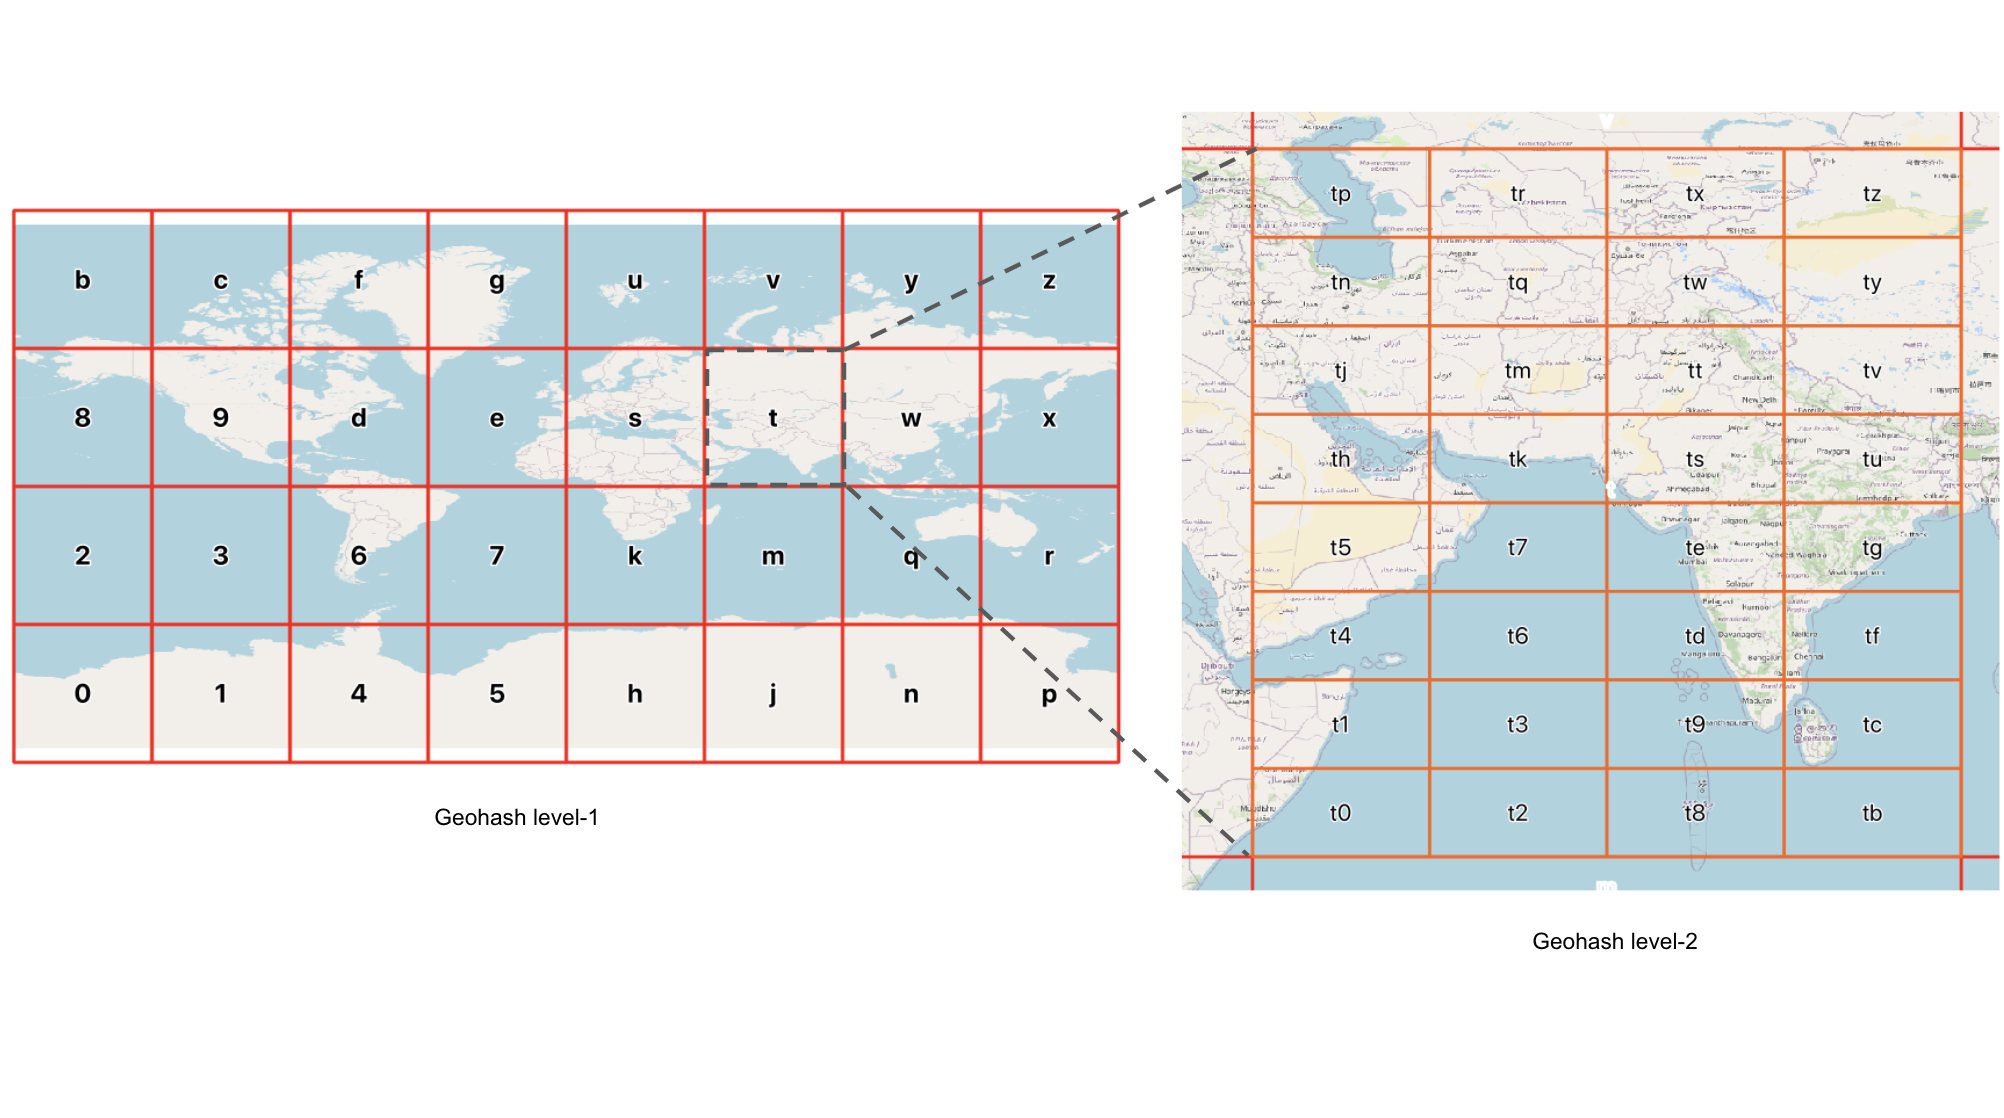
\includegraphics[scale=0.2]{geohash.png}
    \caption{Пример разбиения сферы земли через Geohash на первые 2 префикса}
\end{figure}
  \\
Сам по себе Geohash, как и ниже описанные структуры Uber H3 и S2 - не являются индексами, а лишь методами сериализации геоточек. Реализации алгоритмов поиска на этих методах производится в связке с такими структурами как B-tree, Trie и тд. 

\subsection{1.3.2 Uber H3}
Uber H3 - это сетка гексагональных ячеек (см. рисунок 6), которая используется сериализации и хранения геоданных в приложениях компании Uber, которая, собственно, и разработала данную систему. Каждая ячейка имеет уникальный идентификатор и может быть использована для определения местоположения объектов. Логика работы Uber H3 аналогична логики Geohash за основным исключением, что в Uber H3 используются шестиугольники, а в Geohash - прямоугольники. 
  \\
\begin{figure}[h]
    \centering
    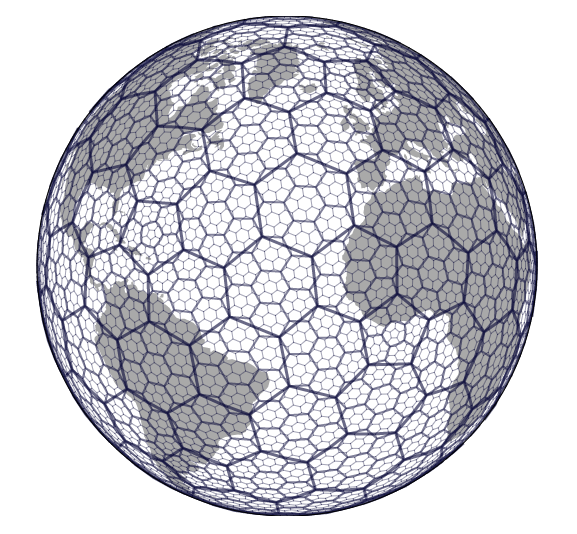
\includegraphics[scale=0.2]{h3.png}
    \caption{Разбиение сферы земли на шестиугольники при использовании H3}
\end{figure}
  \\
Принципиальных отличий между H3 и Geohash, помимо, конечно, разницы в форме - нет. И тот и тот формат в конечном итоге кодирует данные в бинарном виде, имеется возможность перевести данные в строковое представление.  
Важно отметить, что между алгоритмами имееются чисто практические отличия:
\begin{enumerate}
    \item Geohash более прост в реализации. 
    \item Geohash более просто в понимание его человеком
    \item Geohash поддерживается такими СУБД, как: Postgis, Redis, MongoDB
    \item H3 имеет очень обширную библиотеку с дополнительными методами
    \item H3 поддерживается такими СУБД, как: Clickhouse
\end{enumerate}

\subsection{1.3.3 S2 geometry}

S2 Geometry - это библиотека для работы с геометрическими объектами на сфере, разработанная компанией Google. 
  \\
\begin{figure}[h]
    \centering
    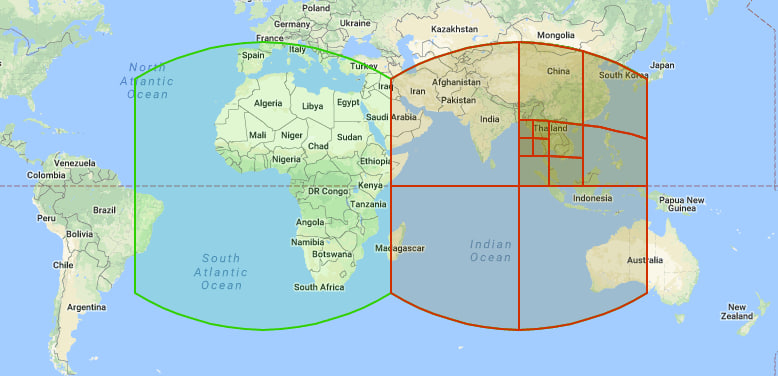
\includegraphics[scale=0.8]{s2-geometry.jpg}
    \caption{Пример разбиения пространства на области с использованием S2 Geometry}
\end{figure}
  \\
Основой S2 Geometry является иерархическая структура данных, называемая S2 Cell. Как показано на рисунке 7, каждая ячейка S2 Cell представляет собой квадрат на сфере, который может быть разбит на более мелкие квадраты более высокого уровня. Уровень ячейки определяется числом n, которое указывает на количество разбиений квадрата на подквадраты. Чем больше значение n, тем меньше размер каждой ячейки.


S2 не имеет значимых качественных или количественных преимуществ перед Geohash и H3. Также, данный алгоритм имеет довольно скудное представление в СУБД, а также в подключаемых библиотеках в различных языках программирования. 
Из-за перечисленных выше причин данный алгоритм не будет далее рассматриваться в этой работе. 